
O controle moderno trata de sistemas multivariáveis, 
não lineares ou variantes no tempo 
de forma mais apropriada do que o controle clássico, 
reduzindo a complexidade das expressões para que 
haja a possibilidade de um processamento satisfatório.
Dentro do universo do controle moderno, 
existe ainda o controle convencional que utiliza a 
análise de sistemas de controle no espaço de estados, 
que utiliza n-equações de primeira ordem 
combinadas em uma equação diferencial vetor-matricial, 
de forma a simplificar e possibilitar 
o trabalho com uma quantidade de variáveis alta 
sem que haja um grande impacto no processamento.  
\cite{Ogata} 
Existem ainda o controle não convencional, 
que também é classificado como controle moderno e que
apresenta uma grande diversidade de técnicas, 
tais como o controle adaptativo, 
algorítmo adaptativo e genético, 
redes neurais, 
as lógicas Fuzzy e Paraconsistente, 
esta última sendo o alvo da abordagem do presente trabalho, 
entre outras.


A lógica, como ramo filosófico que trata das 
relações de coerência racional e discursiva, proposições e conclusões, 
tem como origem a Grécia Antiga com o seu primeiro arranjo formal em 
\emph{Tópicos} de Aristóteles por volta de 340 a.C. 
Apesar de suas bases serem conhecidas e discutidas por 
diversos pensadores anteriores, 
não havia a formalização de uma teoria bem fundada, 
apenas o tratamento de ideias como 
consistência e consequências da contraditoriedade por exemplo. 

Os princípios da lógica enunciadas por Aristóteles são 
basilares para a teoria clássica e 
moldaram o pensamento e a noção de consistência, ou não contraditoriedade, 
estreitamente conectadas ao conceito de completude e 
podem ser descritos formalmente assim:


\begin{enumerate}
\item Princípio de Identidade: 
    \begin{math}
	A \rightarrow B 
	\textrm{ ou } 
	\forall x(x=x);
    \end{math}

\item Princípio do Terceiro Excluído:
    \begin{math}
	A \vee \neg A
	\textrm{ ou }
	\forall x(Ax \vee \neg Ax);
    \end{math}

\item Princípio da Não Contradição: 
    \begin{math}
	\neg (A \wedge \neg A)
	\textrm{ ou }
	\forall x\neg(Ax \wedge \neg Ax).
    \end{math}

\end{enumerate}

O grande desenvolvimento da lógica, 
principalmente nos séculos XIX e XX, 
forneceu ferramental para caracterização e 
tratamento preciso da lógica clássica 
e também possibilitou o desenvolvimento de sistemas lógicos não clássicos, 
rearranjos, experimentações e 
questionamentos de dogmas secularmente estabelecidos.

Uma questão que já havia sido objeto de estudo por diversos pensadores desde os pré-socráticos, 
como Heráclito e sua doutrina da harmonia dos opostos, 
é a questão da contradição, 
que por vezes incomodou-os 
mas que nunca havia sofrido um tratamento formal 
como o desenvolvido por 
Newton C. A. da Costa(1929-presente data) e 
Stanislaw Jaskiwski(1906-1965), 
que propuseram e desenvolveram sistemas lógicos que fossem capazes de lidar com essas inconsistências \cite{DecioKrause}. 





%%%%%%%%%%%%%%%%%%%%%%%%%%%%%%%%%%%%%%%%%%%%%%%%%%%%%%%%%%%
\section{A Lógica Paraconsistente}
%%%%%%%%%%%%%%%%%%%%%%%%%%%%%%%%%%%%%%%%%%%%%%%%%%%%%%%%%%%





Ao restringir-se o princípio da não contradição, 
em um certo sistema lógico, 
obtém-se um resultado que pertence à lógica denominada Paraconsistente, 
desenvolvida por da Costa e Jaskiwski. 

%Para (da Costa e Marconi, 1989), ao restringir em um certo sistema lógico o princípio da não contradição, obtém-se um resultado que pertence à lógica denominada Paraconsistente.


Assim sendo, para uma dada teoria, 
se houver um símbolo de negação, 
como por exemplo "\emph{$\neg $}", 
se em qualquer fórmula fechada \emph{A} não for demonstrável \emph{$A$} e \emph{$\neg A $}, 
a teoria é consistente (não contraditória), 
senão, ela é inconsistente(contraditória).


Teoria é definida por \citeauthor{Gomes2013}(\citeyear{Gomes2013} p.4) como sendo:
\citacao
{
...um conjunto de fórmulas(expressões bem formuladas) de uma linguagem, 
fechadas por uma determinada relação de consequência, 
que caracteriza a lógica subjacente à teoria, 
da qual ela herda todas as suas características estruturais como, 
por exemplo, consistência(não contraditoriedade) e completude.
}

Na lógica clássica, 
uma teoria é completa, 
se e somente se, for consistente para toda a fórmula fechada \emph{A} 
onde \emph{A} e \emph{$\neg A$} é teorema da teoria 
e a teoria é trivial ou supercompleta se todas as fórmulas expressáveis forem demonstráveis, 
tanto \emph{A} quanto \emph{$ \neg A$}.


Sendo que toda a lógica paraconsistente, 
não se pode deduzir qualquer fórmula à partir de uma fórmula \emph{A} e sua negação \emph{$\neg A$}, 
mostrando assim que as noções de inconsistência (contraditoriedade) e trivialidade são de fato independentes.



%A lógica paraconsistente, segundo (Evandro Luis Gomes, 2013) 
%"Apesa do problema da existência de contradições aceitáveis já vir chamando a atenção de lógicos e filósofos pelo menos desde o tempo de Aristóteles, até o aparecimento das lógicas paraconsistentes não se dispunha de um aparato lógico para o estudo das contradiçẽos." 
%Arruda(1990, p.5-6) in Evandro Luis Gomes, 2013 p.5

%"E, como da Costa mesmo reconhecera antes, em 1958, a não trivialidade é que é decisiva ao exercício teórico-racional."
%Evandro Luis Gomes, 2013 p.439



%%%%%%%%%%%%%%%%%%%%%%%%%%%%%%%%%%%%%%%%%%%%%%%%%%%%%%%%%%%%
\subsection{Reticulado de Hasse}
%%%%%%%%%%%%%%%%%%%%%%%%%%%%%%%%%%%%%%%%%%%%%%%%%%%%%%%%%%%%

A Lógica Paraconsistente sendo apropriada para tratar dados inconsistentes foi utilizada em 1987, 
por H. Blair e V. S. Subrahmanian para representar e codificar o funcionamento de bancos de dados inconsistentes. 
\cite{Abe1992} 
Pouco depois Costa, Subrahmanian e Vago propuseram a lógica paraconsistente anotada e sua extensão a uma lógica de predicados paraconsistente anotada de primeira ordem. 

Nas Lógicas Paraconsistentes Anotadas, uma proposição $P$ utiliza um reticulado formado por pares ordenados tal que: 

\begin{center}
\begin{equation}
\tau = \{ ( \mu , \lambda ) \mid \mu ,\lambda \in [0,1] \subset \Re \}
\end{equation}
\end{center}

de acordo com graus de cresça das constantes anotacionais do reticulado de Hasse, 
associado à Lógica Paraconsistente Anotada Evidencial $E\tau$, 
formalmente descritas como 

\begin{center}
\begin{equation}
  \tau = \{ \top , V, F, \bot \}
\end{equation}
\end{center}

os quais descrevem os extremos do reticulado como sendo 
inconsistente,% ($\top$), 
verdadeiro, %(V), 
falso e % (F) e 
paracompleto,% ($\bot$), 
respectivamente, e são representadas conforme Figura \ref{fig:reticuladoHasse}; 

\begin{figure}[!htb]
\caption{Reticulado finito de Hasse}
\center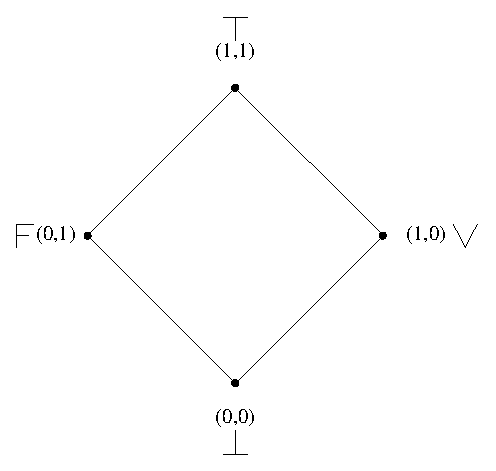
\includegraphics[scale=1.0]{./imagens/C421reticuladoHasse.eps}
\label{fig:reticuladoHasse}

{\small Fonte: \cite{JoaoInacio} }
\end{figure}

Para toda proposição $P$ há um par de valores, chamada de anotação, $(\mu , \lambda )$, onde $\mu$ é o grau de evidência favorável e $\lambda $ é o grau de evidência desfavorável, representada como  $P_{( \mu , \lambda )}$ \cite{Abe2014} .

%$P_{( \mu , \lambda )}$
Como exemplificação, para uma proposição $P \equiv$ \emph{"A velocidade de rotação do motor atingiu o valor desejado."}, assume-se dois especialistas para realizarem a leitura dos valores da anotação. Em um sistema físico, os especialistas geralmente são sensores, como neste caso, poderia ser um encoder ou sensor óptico como contador de voltas associado a uma base de tempo.

\begin{itemize}
\item 
$\mu$ = grau de evidência favorável (especialista 1), ou seja, com quanto de certeza, em um intervalo fechado $[0,1]$, sendo 0 para grau nulo de certeza e 1 grau máximo de certeza para a dada proposição $P$;

\item
$\lambda$ = grau de evidência desfavorável (especialista 2), ou seja, com quanto de certeza, em um intervalo fechado $[0,1]$, sendo 0 o grau nulo de certeza à evidência desfavorável e 1 o grau máximo de certeza à evidência desfavorável para a dada proposição $P$.

\end{itemize}


Assim, podemos interpretar da seguinte forma os valores da anotação para as posições extremas do reticulado finito de Hasse:

\begin{itemize}
\item 
$(\mu, \lambda ) = (1,0)$ : Há um grau de evidência favorável total e um grau de evidencia desfavorável nulo, ou seja, a afirmação da proposição é máxima e sua negação é nula, assim,  $P$ é \emph{Verdadeira} e \emph{A velocidade de rotação do motor atingiu o valor desejado};

\item 
$(\mu, \lambda ) = (0,1)$ : Há um grau de evidência favorável nulo e um grau de evidencia desfavorável máximo, ou seja, a afirmação da proposição é nula e sua negação é máxima, assim,  $P$ é \emph{Falsa} e \emph{A velocidade de rotação do motor não atingiu o valor desejado};

\item 
$(\mu, \lambda ) = (1,1)$ : Há um grau de evidência favorável máximo e também um grau de evidencia desfavorável máximo, ou seja, a afirmação da proposição é máxima e sua negação também é máxima, assim,  $P$ é \emph{Inconsistente} e \emph{A velocidade de rotação do motor atingiu e não atigiu o valor desejado}, contradição;

\item 
$(\mu, \lambda ) = (0,0)$ : Há um grau de evidência favorável nulo e também um grau de evidencia desfavorável nulo, ou seja, a afirmação da proposição é nula e sua negação também é nula, assim,  $P$ é \emph{Indeterminada} e \emph{A velocidade de rotação do motor nem atingiu o valor desejado e nem não atingiu o valor desejado}, situação paracompleta.

\end{itemize}

Os graus de evidência podem assumir valores não extremos:

\begin{itemize}
\item 
$(\mu, \lambda ) = (0.8,0.3)$ : Crê-se com grau de evidência favorável de 80\% e um grau de evidencia desfavorável de 30\%  que \emph{A velocidade rotação do motor atingiu do valor desejado}.
\end{itemize}

\subsubsection{Operações Lógicas}

Algumas operações lógicas booleanas são definidas 
\cite{JISFeAS} \cite{Abe2014}
a partir de duas anotações 
$(\mu _1, \lambda _1)$ e $(\mu _2, \lambda _2)$ 
pertencentes a mesma proposição P, 
aqui denominadas respectivamente $P_1$ e $P_2$:

\begin{itemize}

\item Negação: $\sim$$P _1$ = $(\lambda _1, \mu _1)$ ou 
$\neg$$P _1$ = $(\lambda _1, \mu _1)$

\item Disjunção: $P _1 \vee P _2 = 
(min\{\mu _1, \mu _2\},max\{\lambda _1, \lambda _2\})$ 

\item Conjunção: $P _1 \wedge P _2 = 
(max\{\mu _1, \mu _2\},min\{\lambda _1, \lambda _2\})$ 


\end{itemize}




%%%%%%%%%%%%%%%%%%%%%%%%%%%%%%%%%%%%%%%%%%%%%%%%%%%%%%%%%%%%
\subsection{Quadrado Unitário no Plano Cartesiano - QUPC}
%%%%%%%%%%%%%%%%%%%%%%%%%%%%%%%%%%%%%%%%%%%%%%%%%%%%%%%%%%%%

Uma outra forma de representação da anotação é utilizando o Quadrado Unitário no Plano Cartesiano (QUPC) no qual são transpostos os pontos extremos às respectivas posições de acordo com o par ordenado,  $(\mu, \lambda ) \leftrightarrow (x,y) $, assim o eixo $x$ corresponde ao grau de evidência favorável e o eixo $y$ corresponde ao grau de evidência desfavorável, conforme mostrado na Figura \ref{fig:reticuladoQUPC}.



\begin{figure}[!htb]
\caption{Representação do reticulado no quadrado unitário no plano cartesiano}
\center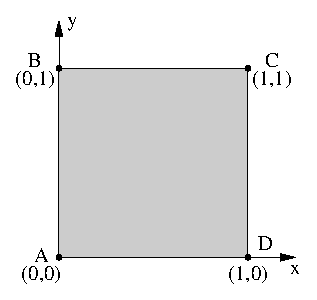
\includegraphics[scale=1.0]{./imagens/C422qupc.eps}
\label{fig:reticuladoQUPC}

{\small Fonte: \cite{JoaoInacio} }
\end{figure}

Os pontos extremos assim representam:

\begin{itemize}
\item $A: (0,0) = \bot \Rightarrow $ Paracompleto;
\item $B: (0,1) = F \Rightarrow $ Falso;
\item $C: (1,1) = \top \Rightarrow $ Contradição;
\item $D: (1,0) = V \Rightarrow $ Verdade.
\end{itemize}

O segmento de reta $\overline{BD}$, entre os pontos referentes às condições $Verdade$ e $Falso$, conforme mostrado na Figura \ref{fig:retaPerfeitamenteDefinida}, é denominada de \emph{Reta Perfeitamente Definida} e dada uma anotação $(\mu, \lambda )$ situada nela, a soma das evidências anotadas é sempre o valor unitário do quadro. 

\begin{figure}[!htb]
\caption{Representação da Reta Perfeitamente Definida}
\center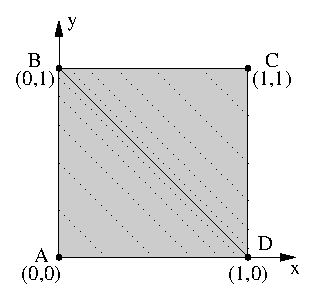
\includegraphics[scale=1.25]{./imagens/C424retaPerfeitamenteDefinida.eps}
\label{fig:retaPerfeitamenteDefinida}

{\small Fonte: \cite{JoaoInacio}}
\end{figure}

A relação dos graus de evidência da anotação quando coincidente à Reta Perfeitamente Definida é: 

\begin{center}
\begin{equation}
\mu + \lambda = 1
\label{eq:evidenciaUnitaria1}
\end{equation}
\end{center}

Assim, temos que:

\begin{center}
\begin{equation}
\mu + \lambda - 1 = 0
\label{eq:evidenciaUnitaria}
\end{equation}
\end{center}


Os graus de evidência não precisam apresentar valores complementares, possuem independência entre si, assim das Equações  
\ref{eq:evidenciaUnitaria1} e 
\ref{eq:evidenciaUnitaria} 
é elaborado o conceito de 
\emph{Grau de Contradição}($G_{ct}$), 
e temos que: 

\begin{center}
\begin{equation}
G _{ct} = \mu + \lambda - 1
\label{eq:grauContradicao}
\end{equation}
\end{center}

pois quanto mais próximo da Reta Perfeitamente Definida, menor é o grau de contradição apresentado pelos graus de evidência, sendo zero quando não houver contradição e o ponto de anotação situar-se sobre a Reta Perfeitamente Definida. 
Quanto mais afastado da Reta Perfeitamente Definida estiver o ponto de anotação, e mais próximo aos pontos A ou C, maior é o Grau de Contradição. 

Quando a anotação estiver situada na região entre os pontos BCD, acima da reta perfeitamente definida, o Grau de Contradição é denominado 
\emph{Grau de Inconsistência} ($G_{it}$), 
e isso ocorre quando, $\mu \ge \lambda $, de forma oposta, quando $\mu < \lambda $ a anotação está situada na região entre os pontos BAD, abaixo da reta perfeitamente definida, e o grau de contradição é denominado 
\emph{Grau de Indefinição} ($G_{id}$), 
então pode-se dizer que:

\begin{center}
\begin{equation}
-1 \le G _{id}  <  0 \le G _{it} \le 1
\label{eq:grauInconsistenciaIndefinicao}
\end{equation}
\end{center}
e
\begin{center}
\begin{equation}
-1 \le G _{ct} \le 1
\label{eq:grauInconsistenciaIndefinicao1}
\end{equation}
\end{center}


O segmento de reta $\overline{ AC }$ , entre os pontos referentes às condições \emph{Paracompleto} e \emph{Contradição}, conforme mostrado na Figura \ref{fig:retaPerfeitamenteIndefinida}, é denominada de \emph{Reta Perfeitamente Indefinida} e dada uma anotação $(\mu, \lambda )$ situada nela, a subtração das evidências anotadas é sempre zero, $\mu = \lambda$, e de forma contrária, quando a anotação está posicionada de forma não coincidente à Reta Perfeitamente Indeterminada, significa que $\mu \neq \lambda$.

\begin{figure}[!htb]
\caption{Representação da Reta Perfeitamente Indefinida}
\center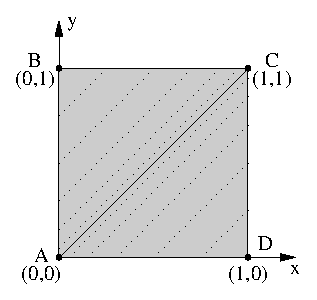
\includegraphics[scale=1.25]{./imagens/C426retaPerfeitamenteIndefinida.eps}
\label{fig:retaPerfeitamenteIndefinida}

{\small Fonte: \cite{JoaoInacio} }
\end{figure}

A relação dos graus de evidência para uma anotação cuja posição coincide com a Reta Perfeitamente Indefinida é: 

\begin{center}
\begin{equation}
\mu - \lambda = 0
\label{eq:evidenciaIndefinida}
\end{equation}
\end{center}

De forma análoga ao Grau de Contradição, da Equação \ref{eq:evidenciaIndefinida} é elaborado o conceito de \emph{Grau de Certeza} ($G _c$), assim temos que: 

\begin{center}
\begin{equation}
G _{c} = \mu - \lambda
\label{eq:grauCerteza}
\end{equation}
\end{center}

Quando os graus de evidência, favorável e desfavorável, são iguais, não há certeza em relação à proposição, mas quando são diferentes, alguma certeza pode ser inferida, até a condição máxima onde uma das evidências é total (1) e a outra é nula (0), caracterizando a condição verdadeira ou falsa, afastando o ponto anotado da Reta Perfeitamente Indefinida. 

Quando a anotação situa-se entre os pontos ABC do QUPC, o grau de certeza é denominado \emph{Grau de Falsidade ($G _f$)}, e tal condição ocorre quando $\mu < \lambda $, caso contrário, se $\mu \ge \lambda $, a anotação situa-se entre os pontos ACD do QUPC, e o grau de certeza é denominado \emph{Grau de Verdade ($G _v)$}, então pode-se dizer que:
\begin{center}
\begin{equation}
-1 \le G _{f}  <  0 \le G _{v} \le 1
\label{eq:grauVerdadeFalsidade}
\end{equation}
\end{center}
e
\begin{center}
\begin{equation}
-1 \le G _{c} \le 1
\label{eq:grauCertezaIntervalo}
\end{equation}
\end{center}

Graficamente são representadas como mostra a Figura \ref{fig:retasgcgct}:

\begin{figure}[!htb]
\caption{Representação dos Graus de Certeza e Contradição em um plano cartesiano}
\center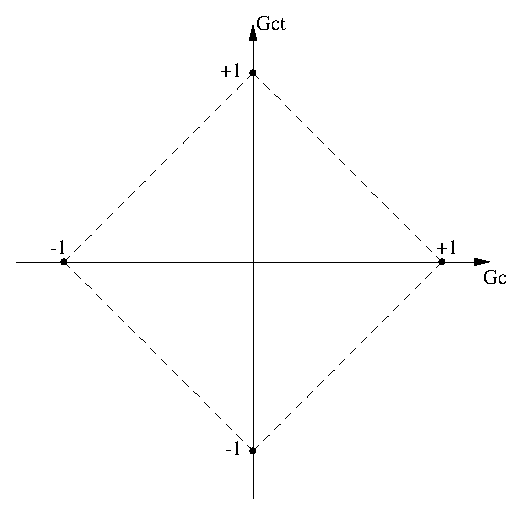
\includegraphics[scale=1.0]{./imagens/C428retasgcgct.eps}
\label{fig:retasgcgct}

{\small Fonte: \cite{JoaoInacio}}
\end{figure}

A representação ainda é dividia em algumas partes, dependendo da aplicação, estabelecendo quais são os limites que definem cada estado, Verdadeiro, Falso, Paracompleto, Contradição e outros mais que forem pertinentes à aplicação, estão representados pelas linhas tracejadas na Figura \ref{fig:valorControle} e são definidos como:

\begin{itemize}
\item \emph{V $_{scc}$ : Valor limite superior de Controle de Certeza};
\item \emph{V $_{icc}$ : Valor limite inferior de Controle de Certeza};
\item \emph{V $_{sci}$ : Valor limite superior de Controle de Incerteza};
\item \emph{V $_{sci}$ : Valor limite inferior de Controle de Incerteza}.

\end{itemize}

\begin{figure}[!htb]
\caption{Representação dos valores de controle}
\center\includegraphics[scale=1.0]{./imagens/C429valorControle.eps}
\label{fig:valorControle}

{\small Fonte: \cite{JoaoInacio}}
\end{figure}

Uma divisão em 12 partes é mostrada na Figura \ref{fig:reticuladoLPA2v} com seus respectivos estados intermediários definidos conforme \citeauthor{JoaoInacio}(\citeyear{JoaoInacio}), sendo 4 regiões extremas:


%\begin{figure}[!htb]
%\center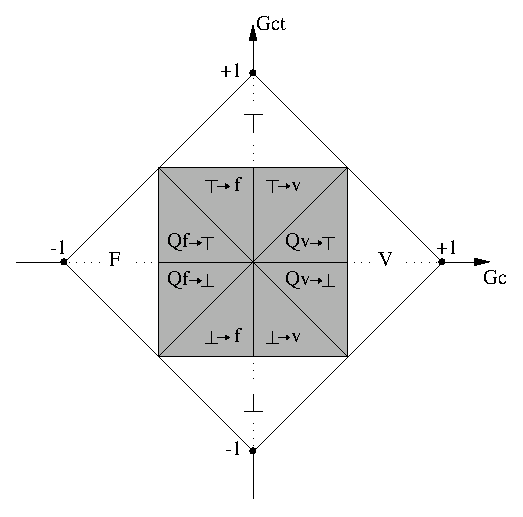
\includegraphics[scale=1.5]{./pic/C430gcgct.eps}
%\caption{Representação do reticulado da LPA2v subdividido em 12 regiões}
%\label{fig:reticuladoLPA2v}
%\end{figure}


\begin{figure}[!h]
\centering
\caption{Representação do reticulado da Lógica $E\tau$ subdividido em 12 regiões}
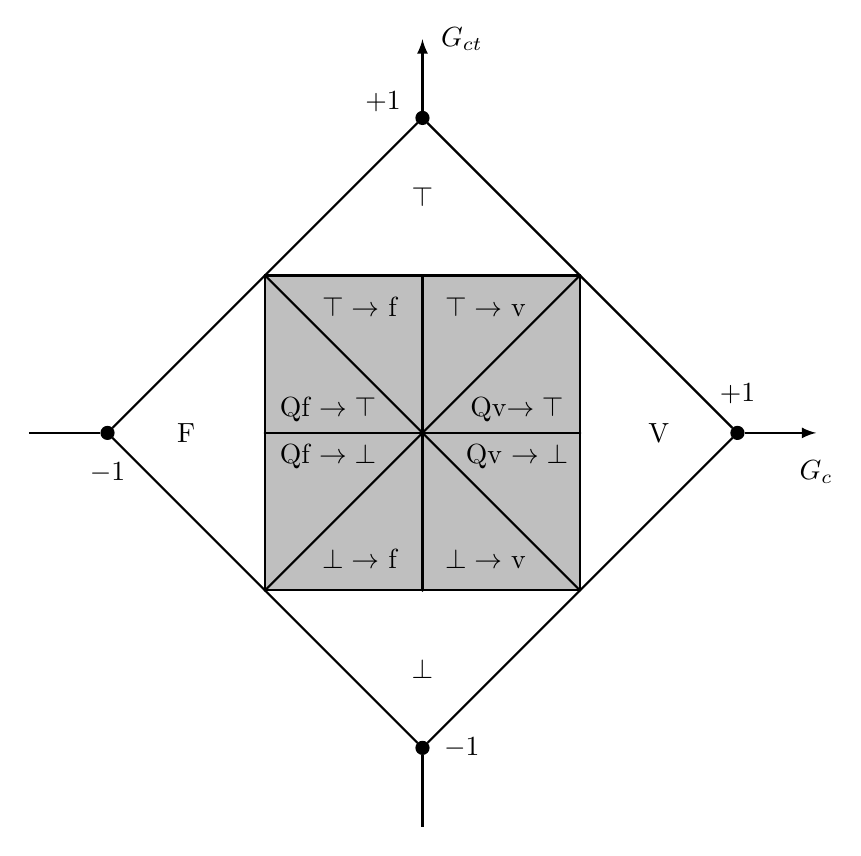
\begin{tikzpicture}[scale=1.0]
\tikzset{ >=latex, inner sep=0pt, outer sep=0pt,  }

%\draw [lightgray, dashed](0,0) grid (10,10);

\node [fill=black, circle] (V) at (9,5) {:};
\node [fill=black, circle] (F) at (1,5) {:};
\node [fill=black, circle] (T) at (5,9) {:};
\node [fill=black, circle] (L) at (5,1) {:};

\node [fill=black, circle] (N) at (5,7) { };
\node [fill=black, circle] (S) at (5,3) { };
\node [fill=black, circle] (E) at (7,5) { };
\node [fill=black, circle] (W) at (3,5) { };

\node [fill=black, circle] (NE) at (7,7) { };
\node [fill=black, circle] (SE) at (7,3) { };
\node [fill=black, circle] (NW) at (3,7) { };
\node [fill=black, circle] (SW) at (3,3) { };


%\draw [dashed] (F) -- (V);
%\draw [dashed] (T) -- (L);
\draw [->, thick] (V)   -- (10,5);
\draw [    thick] (0,5) -- (F);
\draw [->, thick] (T)   -- (5,10);
\draw [    thick] (5,0) -- (L);

\draw [thick] (V) -- (T);
\draw [thick] (T) -- (F);
\draw [thick] (F) -- (L);
\draw [thick] (L) -- (V);

\draw [thick] (N) -- (S);
\draw [thick] (E) -- (W);
\draw [thick] (NE) -- (SW);
\draw [thick] (SE) -- (NW);


\draw[thick] (SW) rectangle (NE);
\fill[nearly transparent] (SW) rectangle (NE);

\node at (8,5) {V};
\node at (2,5) {F};
\node at (5,8) {$\top$};
\node at (5,2) {$\bot$};

\node at (6.2,5.3) {Qv$\rightarrow\top$ };
\node at (6.2,4.7) {Qv $\rightarrow  \bot$ };
\node at (3.8,5.3) {Qf $\rightarrow  \top$ };
\node at (3.8,4.7) {Qf $\rightarrow  \bot$ };
\node at (4.2,6.6) {$\top \rightarrow $ f };
\node at (5.8,6.6) {$\top \rightarrow $ v };
\node at (4.2,3.4) {$\bot \rightarrow $ f };
\node at (5.8,3.4) {$\bot \rightarrow $ v };

\node at (10,4.5) {$G_{c}$};
\node at (5.5,10) {$G_{ct}$};

\node at (4.5,9.2) {$+1$};
\node at (9.0,5.5) {$+1$};
\node at (5.5,1.0) {$-1$};
\node at (1.0,4.5) {$-1$};

\end{tikzpicture}
\label{fig:reticuladoLPA2v}

{\small Fonte: \cite{JoaoInacio} }
\end{figure}




\begin{itemize}
\item V : Verdadeiro;
\item F : Falso;
\item $\top$ : Contradição;
\item $\bot$ : Paracompleto.
\end{itemize}
e 8 regiões intermediárias: 
\begin{itemize}
\item Qv $\rightarrow  \top$ : Quase Verdade tendendo à Contradição;
\item Qv $\rightarrow  \bot$ : Quase Verdade tendendo à  Paracompleto;
\item Qf $\rightarrow  \top$ : Quase Falso tendendo à Contradição;
\item Qf $\rightarrow  \bot$ : Quase Falso tendendo à Paracompleto;
\item $\top \rightarrow $ f : Contradição tendendo à Falso;
\item $\top \rightarrow $ v : Contradição tendendo à Verdadeiro;
\item $\bot \rightarrow $ f : Paracompleto tendendo à Falso;
\item $\bot \rightarrow $ v : Paracompleto tendendo à Verdadeiro.

\end{itemize}

O reticulado subdividido em 12 regiões como mostrado, é aplicado em situações nas quais a tomada de decisão utiliza estados discretos bem definidos para atuação, onde para cada posição da anotação e respectivamente um estado do reticulado, uma ação é tomada, assim sendo, a quantidade de subdivisões está fortemente dependente da aplicação.


O reticulado pode ser dividido de outras formas, dependendo dos limites dos Graus de Certeza e Contradição que o sistema permite. A Figura \ref{fig:reticuladoLPA2v2} mostra uma das possibilidades com a representação de 8 regiões do reticulado. 


\begin{figure}[!h]
\centering
\caption{Representação do reticulado da Lógica $E\tau$ subdividido em 8 regiões}
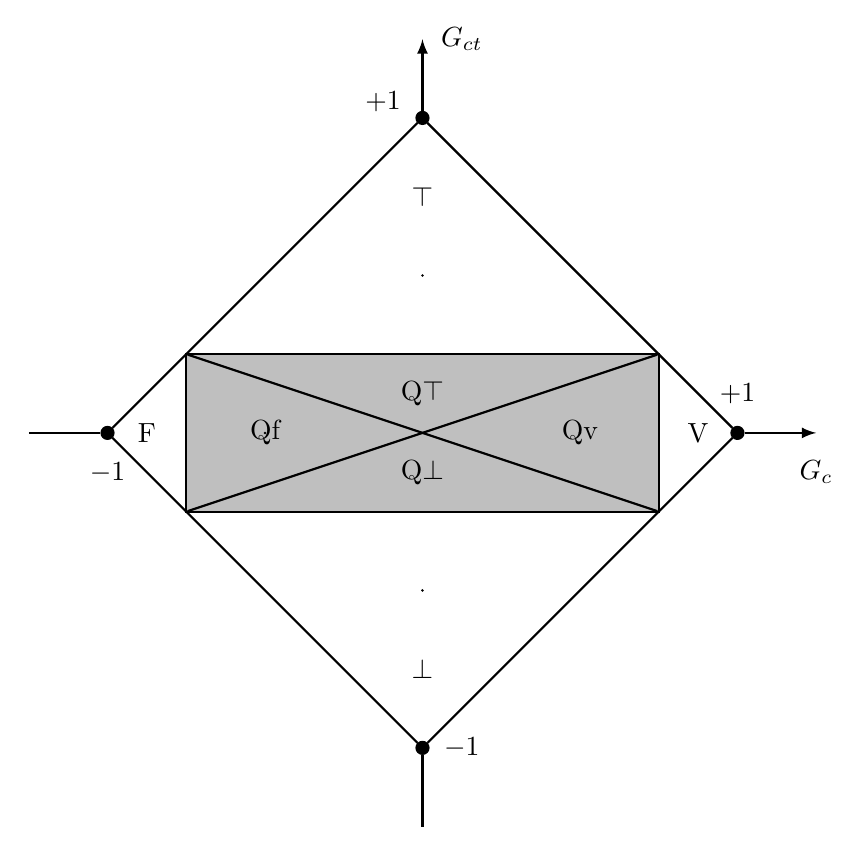
\begin{tikzpicture}[scale=1.0]
\tikzset{ >=latex, inner sep=0pt, outer sep=0pt,  }

%\draw [lightgray, dashed](0,0) grid (10,10);

\node at (10,4.5) {$G_{c}$};
\node at (5.5,10) {$G_{ct}$};

\node at (4.5,9.2) {$+1$};
\node at (9.0,5.5) {$+1$};
\node at (5.5,1.0) {$-1$};
\node at (1.0,4.5) {$-1$};

\node [fill=black, circle] (V) at (9,5) {:};
\node [fill=black, circle] (F) at (1,5) {:};
\node [fill=black, circle] (T) at (5,9) {:};
\node [fill=black, circle] (L) at (5,1) {:};

\node [fill=black, circle] (N) at (5,7) { };
\node [fill=black, circle] (S) at (5,3) { };
\node [fill=black, circle] (E) at (7,5) { };
\node [fill=black, circle] (W) at (3,5) { };

\node [fill=black, circle] (NE) at (8,6) { };
\node [fill=black, circle] (SE) at (8,4) { };
\node [fill=black, circle] (NW) at (2,6) { };
\node [fill=black, circle] (SW) at (2,4) { };

\draw [->, thick] (V)   -- (10,5);
\draw [    thick] (0,5) -- (F);
\draw [->, thick] (T)   -- (5,10);
\draw [    thick] (5,0) -- (L);

\draw [thick] (V) -- (T);
\draw [thick] (T) -- (F);
\draw [thick] (F) -- (L);
\draw [thick] (L) -- (V);

\draw [thick] (NE) -- (SW);
\draw [thick] (SE) -- (NW);

\draw[thick] (SW) rectangle (NE);
\fill[nearly transparent] (SW) rectangle (NE);

\node at (8.5,5.0) {V};
\node at (1.5,5.0) {F};
\node at (5.0,8.0) {$\top$};
\node at (5.0,2.0) {$\bot$};

\node at (7.0,5.0) {Qv};
\node at (3.0,5.0) {Qf};
\node at (5.0,5.5) {Q$\top$};
\node at (5.0,4.5) {Q$\bot$};

\end{tikzpicture}
\label{fig:reticuladoLPA2v2}

{\small Fonte: Próprio autor}
\end{figure}

Sendo 4 regiões extremas,
\begin{itemize}
\item V : Verdadeiro;
\item F : Falso;
\item $\top$ : Contradição;
\item $\bot$ : Paracompleto.
\end{itemize}
e 4 regiões intermediárias: 
\begin{itemize}
\item Qv: Quase Verdade;
\item Qf: Quase Falso;
\item Q$\top$: Quase Contradição;
\item Q$\bot$: Quase Paracompleto.

\end{itemize}


%###

É possível e desejável que se possa utilizar um valor resultante que exclua os efeitos das incertezas ou contradições, 
como é citado por 
\citeauthor{JairJoaoGermano}(\citeyear{JairJoaoGermano}): 
\begin{citacao}
{
"Um sistema de decisão capaz de analisar dados originários de Conhecimento Incerto terá maior robustez quando, 
ao final da análise,
apresentar um resultado que represente o valor de certeza puro, 
isto é, não contaminado pelos efeitos das incertezas."
}
\end{citacao}

O valor que elimina o efeito da incerteza é denominado \emph{Grau de Certeza Real - G$_{CR}$} 
e é calculado pela distância (D) do Ponto de análise, $(G_c,G_{ct})$, 
em relação ao ponto de máximo Grau de Certeza $V$, 
no vértice direito do reticulado, 
conforme mostrado na Figura \ref{fig:reticuladoGer}.


\begin{figure}[!h]
\centering
\caption{Representação do Grau de Certeza Real no reticulado }
\begin{tikzpicture}[scale=1.0]
\tikzset{ >=latex, inner sep=0pt, outer sep=0pt,  }

%\draw [lightgray, dashed](0,0) grid (10,10);

\node at (10,4.5) {$G_{c}$};
\node at (5.5,10) {$G_{ct}$};

\node at (4.5,9.2) {$+1$};
\node at (9.0,5.5) {$+1$};
\node at (5.5,1.0) {$-1$};
\node at (1.0,4.5) {$-1$};

\node at (9.0,4.5) {V};
\node at (1.0,5.5) {F};
\node at (5.5,9.0) {$\top$};
\node at (4.5,1.0) {$\bot$};

\node [fill=black, circle] (V) at (9,5) {:};
\node [fill=black, circle] (F) at (1,5) {:};
\node [fill=black, circle] (T) at (5,9) {:};
\node [fill=black, circle] (L) at (5,1) {:};

\draw [thick] (V) -- (T);
\draw [thick] (T) -- (F);
\draw [thick] (F) -- (L);
\draw [thick] (L) -- (V);

\draw [->, thick] (V)   -- (10,5);
\draw [    thick] (0,5) -- (F);
\draw [->, thick] (T)   -- (5,10);
\draw [    thick] (5,0) -- (L);

\draw [lightgray,dashed] (V) -- (F);
\draw [lightgray,dashed] (T) -- (L);

\node [fill=black, circle] (P) at (6.0,7.0) {:};
\node [fill=gray,  circle] (p) at (5.4,5.0) [gray] {:};
\node [fill=black, circle] (r) at (6.0,5.0) [gray]{.};

\draw [blue,ultra thick] (P) -- (V);
\draw [green ] (r) -- (V);
\draw [yellow] (P) -- (r);
%\draw [green,ultra thick] (9.0,4.9) -- (5.4,4.9);

\draw [red, ultra thick,<-]  (p) to [out=85, in=236] (P);

\node at (7.0,6.0) [blue]{D};
\node at (5.7,7.4) {($G_c$,$G_{ct}$)};
\node at (5.5,4.6) {$G_{CR}$};

\end{tikzpicture}
\label{fig:reticuladoGer}

{\small Fonte: \cite{JairJoaoGermano}}
\end{figure}


O Grau de Certeza Real ($G_{CR}$) 
é calculado utilizando o Teorema de Pitágoras para achar a distância D 
conforme Equação \ref{eq:grauCertezaReal}. 

\begin{center}
\begin{equation}
D = \sqrt{(1-|G_c|)^2+G_{ct}^2}
\label{eq:grauCertezaReal}
\end{equation}
\end{center}

Para valores de $G_c \geq 0$: 

\begin{center}
\begin{equation}
G_{CR} = (1-D)
\end{equation}
\end{center}

Para valores de $G_c < 0$:

\begin{center}
\begin{equation}
G_{CR} = (D-1)
\end{equation}
\end{center}


O Grau de Evidência Real é representado por $\mu_{ER}$ 
e é utilizado para converter o $Gc$ ou $G_{CR}$ 
em uma variável dentro do intervalo fechado $[0,1]$, 
permitindo que o resultado de um bloco LPA$E\tau$ 
possa ser utilizado como entrada em outro bloco. 
Para a conversão é efetuada a equação \ref{eq:muer}:

\begin{equation}
\mu_{ER} = \frac{Gc + 1}{2}
\label{eq:muer}
\end{equation}


Tanto o Grau de Certeza Real quanto o Grau de Evidência Real 
ou os estados ou regiões do reticulado 
podem ser utilizados para realizar o controle dos mais diversos tipos de sistemas, 
dependendo apenas do tipo de controle e de sistema que deve ser implementado. 

%%%%%%%%%%%%%%%%%%%%%%%%%%%%%%%%%%%%%%%%%%%%%%%%%%%%%%%%%%%%
\subsection{A Lógica $E\tau$ e suas aplicações}
%%%%%%%%%%%%%%%%%%%%%%%%%%%%%%%%%%%%%%%%%%%%%%%%%%%%%%%%%%%%

Os Sistemas Inteligentes estão cada vez mais presentes 
em diversas aplicações modernas, 
e segundo \citeauthor{JISF2011}(\citeyear{JISF2011}), 
há um predomínio de Lógicas Não-Clássicas no suporte à tomada de decisão desses sistemas. 
O sucesso na aplicação de técnicas como a Lógica $E\tau$, 
que é uma extensão da Lógica Paraconsistente Anotada, 
se dá em grande medida pelo uso de 
algorítmos baseados em estudos dos reticulados representativos e 
efetiva tradução matemática 
gerando um modelo eficiente aplicado em situações reais.

Assumindo que a lógica filosófica trata da descrição formal da linguagem natural 
e define a sua estrutura de declaração, então, 
sendo encontrada a linguagem adequada 
é possível traduzir o raciocínio formal em LPA, 
modelando raciocínios com a possibilidade de 
tratar contradições ou incoerências, 
e trabalhar com situações reais, 
da mesma forma que o Modelo Clássico, 
que aplica regras computacionais, 
a Lógica $E\tau$ possui um conjunto de axiomas e regras de inferência 
que possibilitam um raciocínio válido em situações reais.

\subsubsection{Robótica}

Os algorítmos baseados no estudo do Reticulado Representativo gera 
Estados Lógicos Paraconsistentes através da 
descrição do algorítmo Para-Analisador da Lógica $E\tau$, 
possibilitando que o sistema receba informação 
através dos graus de evidência ($\mu, \lambda$), 
processe os graus de certeza e contradição ($G_c$ e $G_{ct}$) e 
chegue a uma conclusão, de alta contradição e busque por mais dados ou 
um alto grau de certeza, que de um modo geral, implica em tomar uma ação. 

Os Graus de Certeza e Contradição podem gerar um Grau de Certeza Real, 
que pode servir de entrada para outra célula ou 
Nó de Análise Paraconsistente (NAP), 
possibilitando uma rede de análises para a tomada de decisão,
como apresentado na construção e aperfeiçoamentos realizados no Robô Emmy,
\cite{JoaoInacio}\cite{ClaudioRodrigoTorres} 
desenvolvendo e aplicando tais técnicas aplicadas ao sistema de movimentação.

\subsubsection{Engenharia de Produção}

A Lógica $E\tau$ pode ser aplicada em diversas áreas 
sendo um outro exemplo a sua aplicação na 
área de Eng. de Produção, 
como é mostrado no artigo de 
\citeauthor{FabioIsraelJair}(\citeyear{FabioIsraelJair}), 
que mostram um estudo para avaliação do projeto de uma fábrica, 
como são selecionadas as variáveis relevantes, ou fatores, como são chamados,
níveis de exigência para tomada de decisão, 
atribuição de pesos aos fatores de decisão, 
para obtenção dos graus de crença e descrença. 
Construção de uma base de dados, sua pesquisa e obtenção dos resultados.
Análise dos resultados e fidedignidade utilizando um 
Método de Análise pelo Baricentro.

\subsubsection{Logística}

No segmento logístico pode-se citar a dissertação do 
Profº Me. Vander Célio Nunes (\cite{Vander}), 
que aplicou a Lógica $E\tau$ ao processo de paletização 
através da medição de peças e do tratamento de incertezas 
relacionadas a possibilidade de seu depósito ou encaixe na pilha de palets, 
levando à otimização de cargas armazenadas em um determinado espaço. 
O seu trabalho, utilizando uma célula de manufatura 
com um braço robótico industrial, 
permite a extrapolação da sua aplicação para portos e armazens de containers.



\subsubsection{Medicina}

Em aplicações de apoio à medicina através de algoritmos para 
auxílio de diagnóstico de patologias como em 
\citeauthor{MauricioCM}(\citeyear{MauricioCM}), 
onde a Lógica Paraconsistente é aplicada na análise de mamografias.


\subsubsection{Sistema de Controle Híbrido}

No segmento de controle, a Lógica $E\tau$ é utilizada em conjunto com um 
sistema Proporcional-Integral - PI de modo que 
as ações convencionais são executadas pelo bloco PI, 
mas são estruturadas utilizando a Lógica $E\tau$ no 
tratamento dos sinais externos. 
A implementação é feita por 
\citeauthor{Marcelo}(\citeyear{Marcelo}) 
em uma planta de controle de nível e um
controlador lógico programável. 
O sistema Híbrido é posto em operação e 
comparado com técnicas consagradas como o 
controle puramente PI, ajustado com o
método de Ziegler-Nichols e com o 
método interno do controlador. 




%%%%%%%%%%%%%%%%%%%%%%%%%%%%%%%%%%%%%%%%%%%%%%%%%%%%%%%%%%%%
%%%%%%%%%%%%%%%%%%%%%%%%%%%%%%%%%%%%%%%%%%%%%%%%%%%%%%%%%%%%




